\documentclass{article}
\usepackage[margin=1.0in]{geometry}
\usepackage{amsmath, amssymb, mathrsfs}
\usepackage[english]{babel}
\usepackage{graphicx}
\usepackage{enumerate}
\usepackage{listings}
\usepackage{tikz}
\renewcommand{\vec}[1]{\mathbf{#1}}
\newcommand{\floor}[1]{\left\lfloor #1 \right\rfloor}
\newcommand{\ceil}[1]{\left\lceil #1 \right\rceil}

\title{Machine Learning from Data Assignment 7}
\author{Greg Stewart}
\date{\today}

\begin{document}

\maketitle

\subsection*{Classifying Handwritten Digits}

\begin{enumerate}[(a)]
  \item \textit{Give separate plots of the training and test data, together with the separators.}

    On the \textbf{left} is the training data, and on the \textbf{right} is the test data:

    \begin{center}
    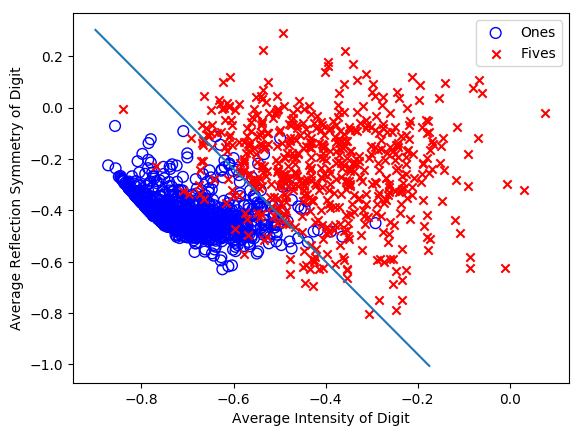
\includegraphics[width=.45\textwidth]{./data/trainingplot.png}
    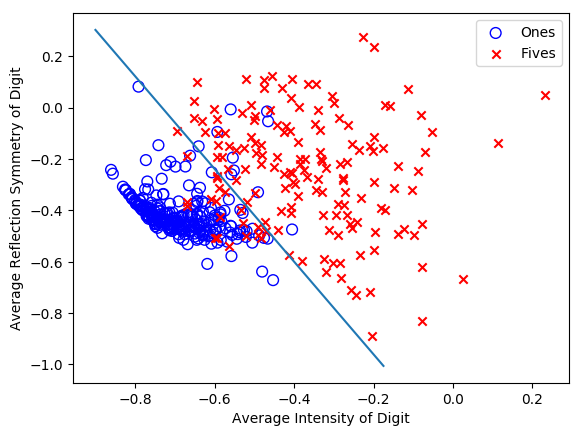
\includegraphics[width=.45\textwidth]{./data/testplot.png}
    \end{center}

  \item \textit{Compute $E_{in}$ on your training data and $E_{test}$, the test error on the test
    data.}

    $E_{in} = 0.05061 = 5.061\%$

    $E_{test} = 0.07311 = 7.311\%$

  \item \textit{Obtain a bound on the true out-of-sample error. You should get two bounds, one 
    based on $E_{in}$ and one based on $E_{test}$. Use a tolerance $\delta = 0.05$.
    Which is the better bound?}

    Using $E_{in}$, we have

    \begin{align*}
      E_{out} &\leq E_{in} + \sqrt{\frac{8}{N}\ln\frac{4(2N)^{d_{VC}} + 4}{\delta}} \\
      &\leq 0.05061 + \sqrt{\frac{8}{1561}\ln\frac{4(2\cdot1561)^{3} + 4}{0.05}} \\
      &\leq .05061 + .38232 = .43293 \\
      &\leq 43.3\%
    \end{align*}

    and using $E_{test}$, we have
    
    \begin{align*}
      E_{out} &\leq E_{test} + \sqrt{\frac{1}{2N}\ln\frac{2M}{\delta}} \\
      &\leq .07311 + \sqrt{\frac{1}{2\cdot424}\ln\frac{2}{.05}} = .07311 + 0.06596\\
      &\leq 13.91\%
    \end{align*}

    Obviously, the bound obtained from $E_{test}$ is the better of the two.

  \item \textit{Now repeat using a 3rd order polynomial transform.}
    
    On the \textbf{left} is the training data, and on the \textbf{right} is the test data:

    \begin{center}
      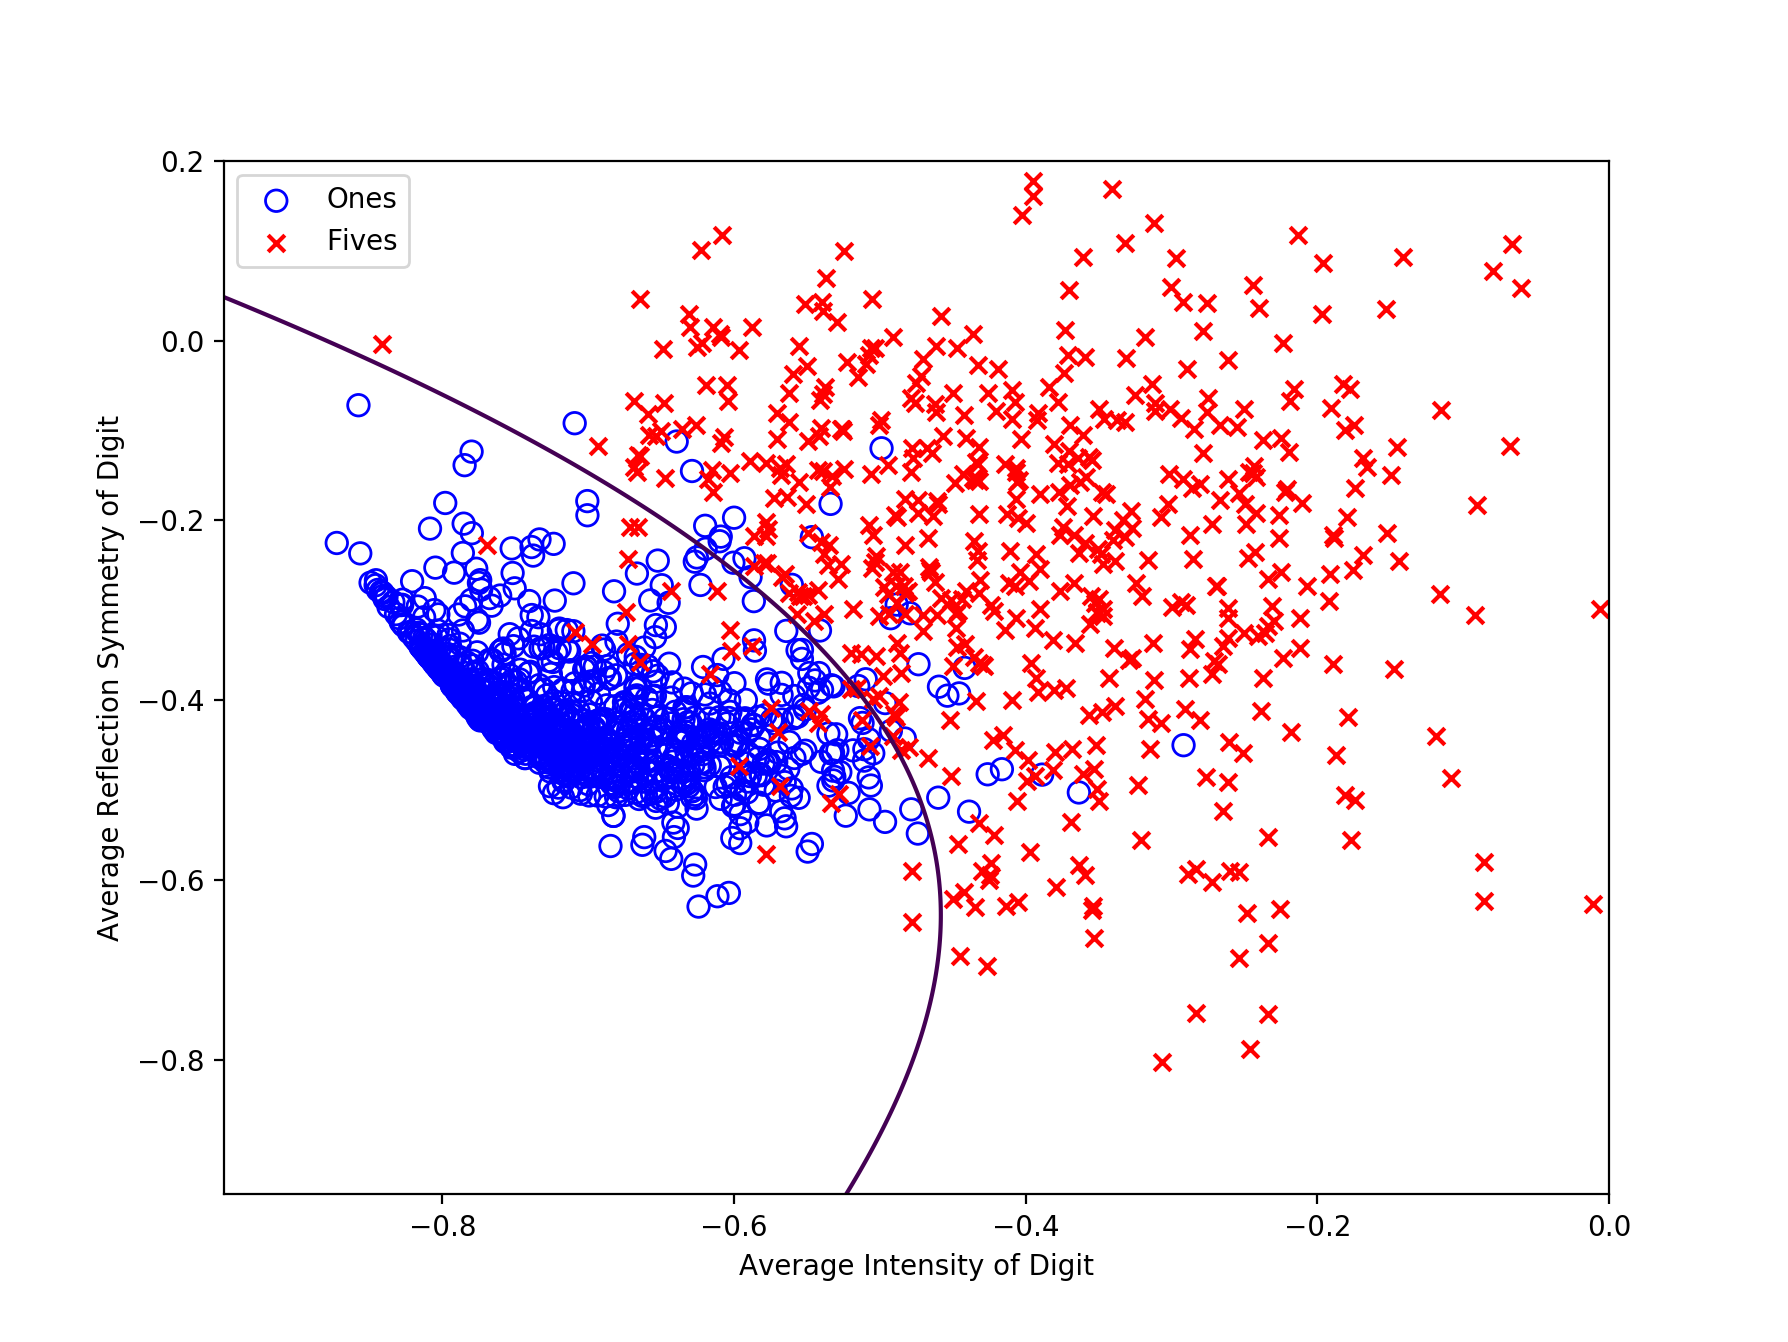
\includegraphics[width=.45\textwidth]{3rdtrans.png}
      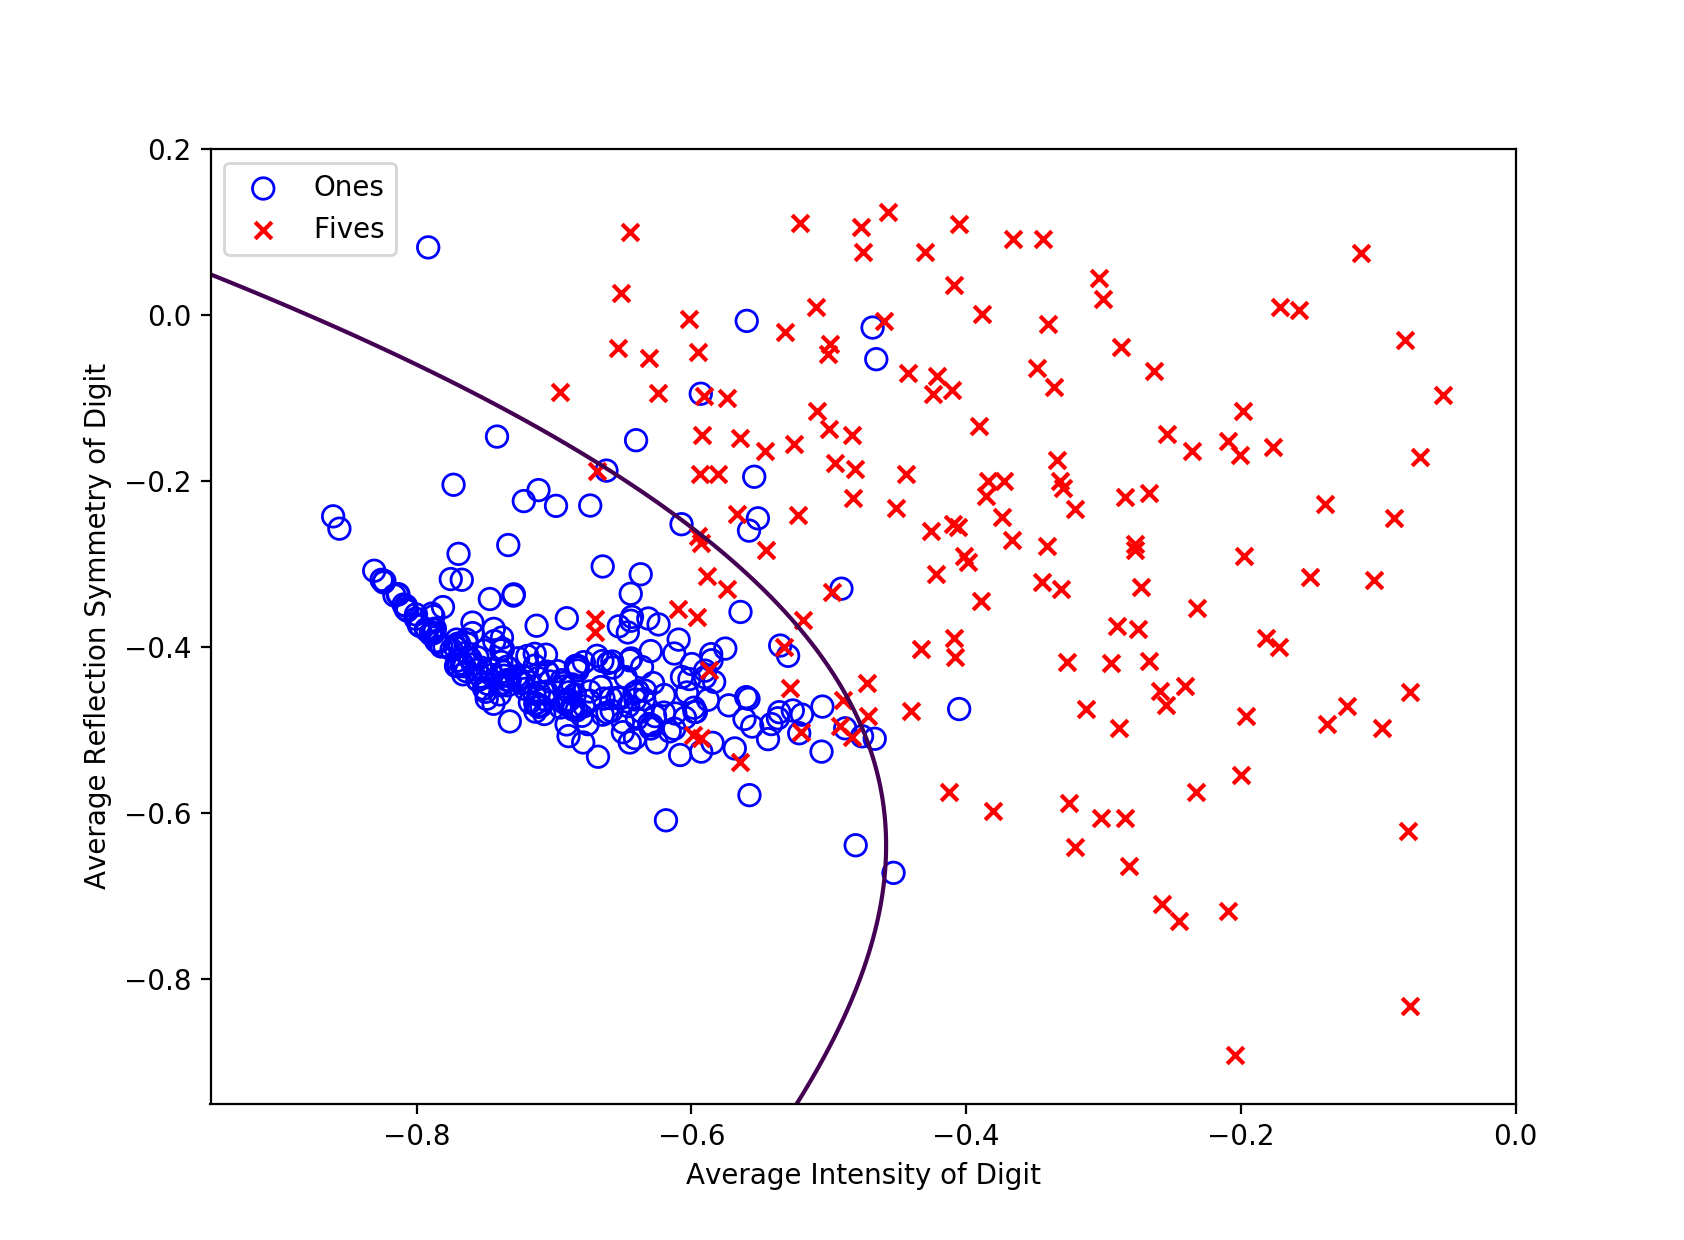
\includegraphics[width=.45\textwidth]{3rdEtest.png}
    \end{center}

    $$E_{in} = 0.04228 = 4.228\% \qquad\qquad\qquad\qquad E_{test} = 0.07547 = 7.547\%$$

    The error bars are as follows.

    \begin{align*}
      E_{out} &\leq E_{in} + \sqrt{\frac{8}{N}\ln\frac{4(2N)^{d_{VC}} + 4}{\delta}} \\
      &\leq 0.04228 + \sqrt{\frac{8}{1561}\ln\frac{4(2\cdot1561)^{10} + 4}{0.05}} \\
      &\leq .04228 + .65941 = .70169 \\ 
      &\leq 70.17\%
    \end{align*}

    and using $E_{test}$, we have
    
    \begin{align*}
      E_{out} &\leq E_{test} + \sqrt{\frac{1}{2N}\ln\frac{2M}{\delta}} \\
      &\leq .07547 + \sqrt{\frac{1}{2\cdot424}\ln\frac{2}{.05}} = .07547 + 0.06596\\
      &\leq 14.14\%
    \end{align*}
    
  \item \textit{As your final deliverable to a customer, would you use the linear model with or 
    without the 3rd order polynomial transform? Explain.}

    I'd deliver the linear model without a 3rd order transform to the customer. It has a very
    slightly lower bound for $E_{out}$, and is simpler, so it's less at risk for overfitting,
    unlike the 3rd order transform, which certainly is at risk. For the unsatisfied customer,
    though, the 3rd order transform result could be delivered if they are incredulous about
    the simplicity of the linear result, then quickly snatched away again, like a cruel aunt 
    teasing her toddler nephew with a piece of candy.

\end{enumerate}


\subsection*{Gradient Descent on "Simple" Function}

\textit{Consider} $$f(x,y) = x^2 + 2y^2 + 2\sin{(2\pi x)}\sin{(2\pi y)}$$

\begin{enumerate}[(a)]
  \item \textit{Implement gradient descent to minimize using the given starting values and
    learning rate. Number of iterations = 50. Give a plot of how the function value drops with
    the number of iterations performed. Repeat for $\eta = 0.1$}

    The two plots are
    
    \begin{center}
      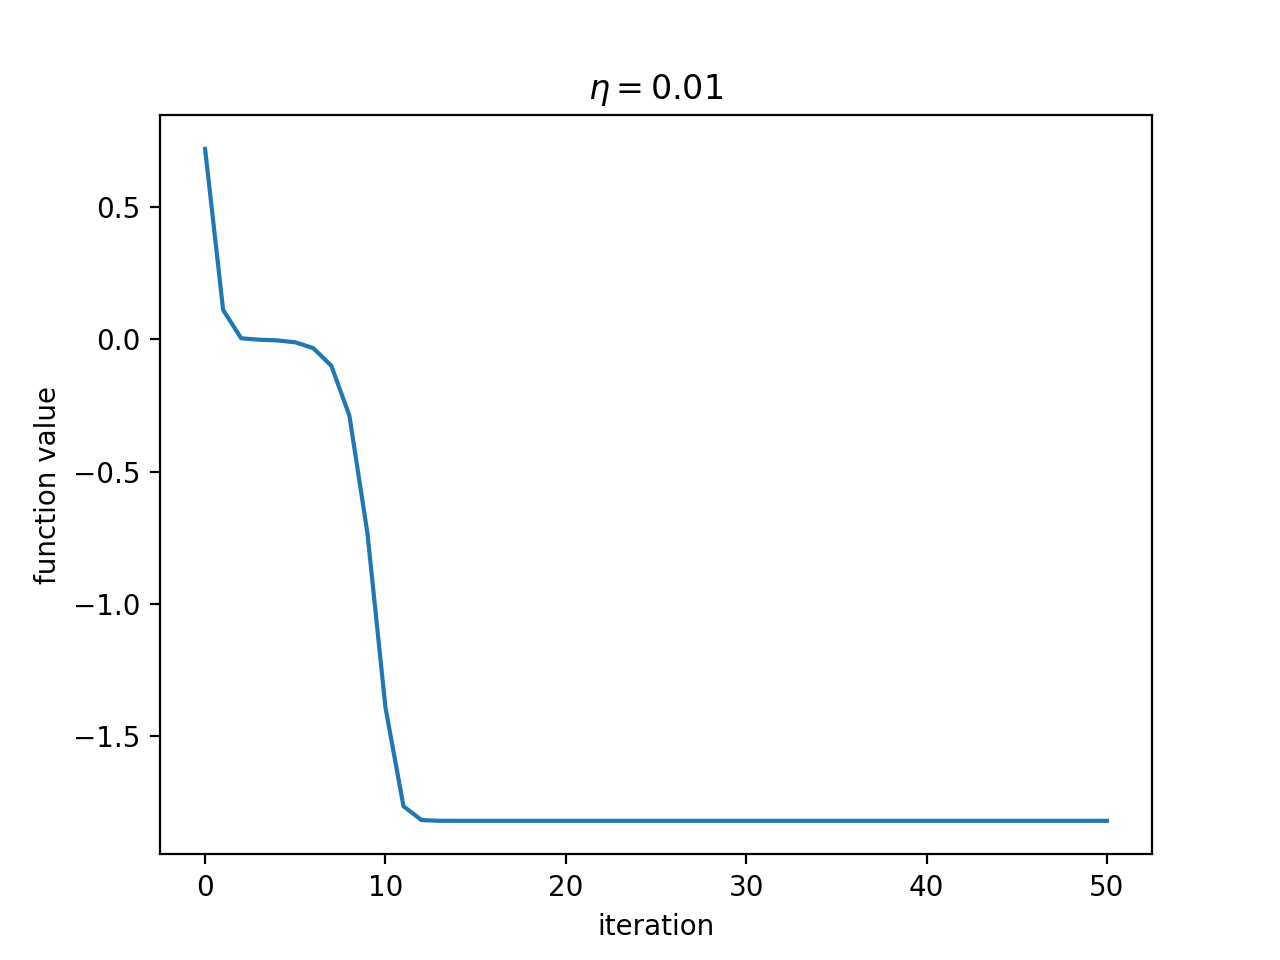
\includegraphics[width=.45\textwidth]{2asmalleta.png}
      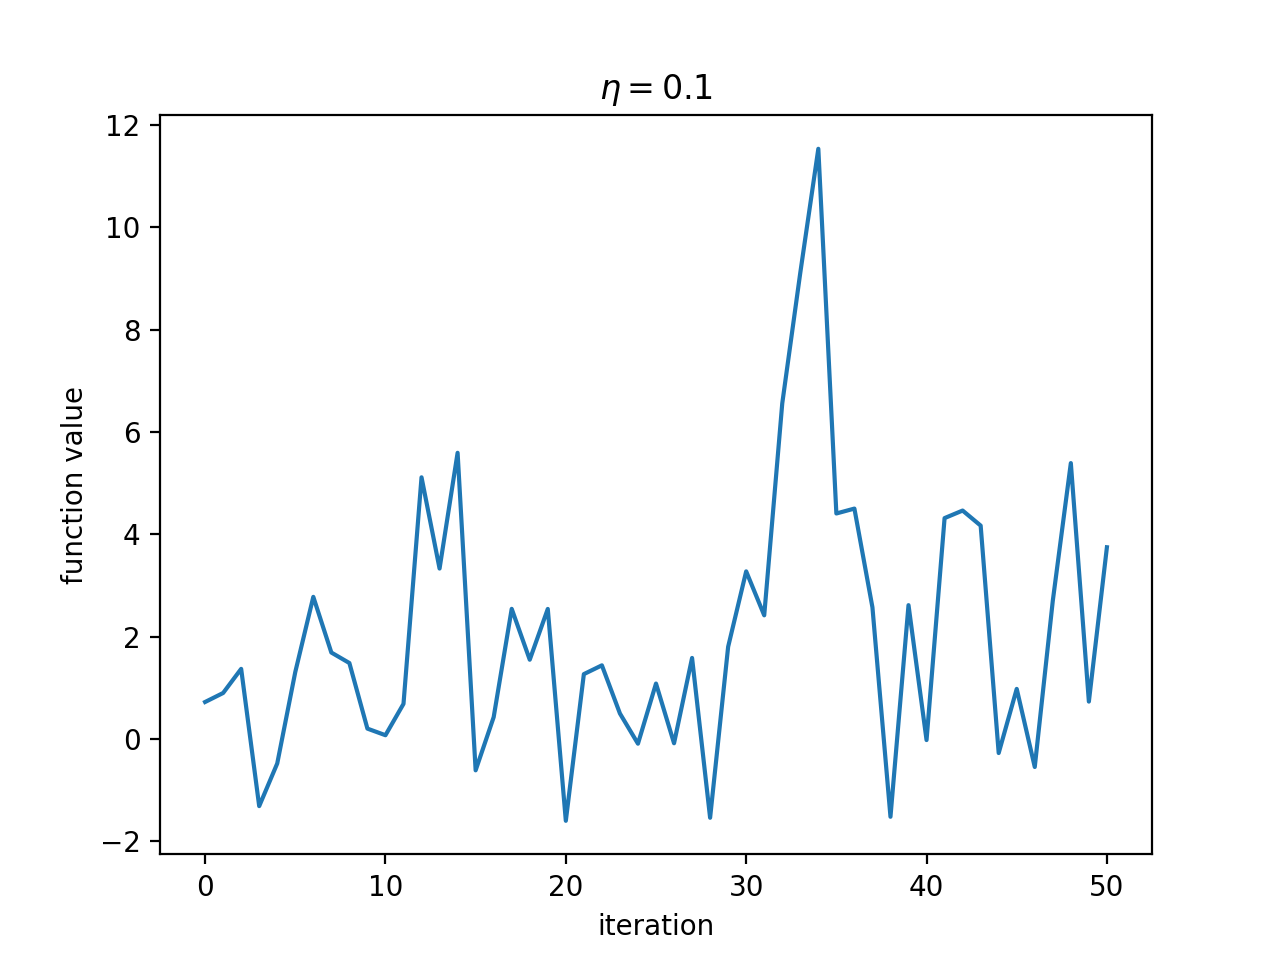
\includegraphics[width=.45\textwidth]{2abigeta.png}
    \end{center}

    Clearly, the larger learning rate caused the descent algorithm to overshoot, and it couldn't
    come back from it, perhaps entering a region with another local minimum or something like that.

  \item \textit{Do the same for the given pairs of points and the better $\eta$.}

    \begin{center}
      \begin{tabular}{c | c c}
        $(x_0, y_0)$ & $(x_f, y_f)$ & $f(x_f, y_f)$ \\[0.5ex]
        \hline
        $(0.1,0.1)$ & $(0.243,-0.238)$ & $-1.82$ \\
        $(1.0,1.0)$ & $(1.218,0.713)$ & $0.593$ \\
        $(-0.5,-0.5)$ & $(-0.731,-0.238)$ & $-1.33$ \\
        $(-1.0,-1.0)$ & $(-1.218,-0.713)$ & $0.593$ \\
      \end{tabular}
    \end{center}

\end{enumerate}


\subsection*{Problem 3.16}

\textit{Concerned with using logistic regression to get hard classification using risk matrix.
The final hypothesis is $$g(\vec{x}) = \mathbb{P}[y = +1 \mid \vec{x}],$$ which is the estimate
of the probability that $y = +1$. The cost matrix is given by
\begin{center}
  \begin{tabular}{c c | c c}
     & & True & Classification \\
     & & +1 (correct person) & -1 (intruder) \\
     \hline
     you & +1 & 0 & $c_a$ \\
     say & -1 & $c_r$ & 0 \\
  \end{tabular}
\end{center}
For a fingerprint $\vec{x}$, $g(\vec{x})$ needs to be computed and used to decide acceptance or
rejection. Accept if $g(\vec{x}) \geq \kappa$, where $\kappa$ is the threshold.}

\begin{enumerate}[(a)]
  \item \textit{Define cost(accept) as your expected cost if you accept the person. Also define
    cost(reject). Show 
    \begin{align*}
      cost(accept) &= (1-g(\vec{x}))c_a \\
      cost(reject) &= g(\vec{x})c_r
    \end{align*}}

    The cost of accepting 1 person if they ought be accepted is of course 0, and $c_a$ if it's
    an intruder. Since $g(\vec{x})$ is defined as the chance of $y$ being +1 (acceptance) given
    the fingerprint. The cost(accept), or expectation of cost, is then given by the probability
    of each event given \textit{you} accept multiplied by the cost:

    $$cost(accept) = g(\vec{x})\cdot0 + (1 - g(\vec{x}))c_a = (1-g(\vec{x}))c_a.$$

    The expected cost of rejection is calculated the same way:

    $$cost(reject) = g(\vec{x})c_r + (1-g(\vec{x}))\cdot0 = g(\vec{x})c_r.$$

  \item \textit{Use part (a) to derive a condition on $g(\vec{x})$ for accepting the person and
    hence show that $$\kappa = \frac{c_a}{c_a + c_r}.$$}

    We want cost(accept) - cost(reject) $\leq 0$. So we can write

    \begin{align*}
      (1-g(\vec{x}))c_a - g(\vec{x})c_r &\leq 0 \\
      c_a - (c_a + c_r)g(\vec{x}) &\leq 0 \\
      c_a &\leq (c_a + c_r)g(\vec{x}) \\
      \frac{c_a}{c_a + c_r} &\leq g(\vec{x})
    \end{align*}

    so we have a threshold for $g(\vec{x})$, given by $\frac{c_a}{c_a + c_r}$, meaning that for
    $\kappa$ we have 

    $$\kappa = \frac{c_a}{c_a+c_r}$$

  \item \textit{Use cost matrices for the supermarket and CIA applications in example 1.1 to
    compute the threshold $\kappa$ for each of these two cases. Give some intuition for the 
    threshold you get.}

    \begin{enumerate}[i.]
      \item Supermarket.
        
        $\kappa = \frac{1}{1+10} = .090909...$

      \item CIA

        $\kappa = \frac{1000}{1000+1} = 0.999001$

    \end{enumerate}

    These are not very surprising values. In the CIA, you'd essentially never want to have a 
    false positive---admitting an intruder could be detrimental, so the threshold for acceptance
    should be very high. A false rejection is merely an inconvenience in this case.

    Conversely, the threshold for acceptance for the supermarket is very low. It's not worth 
    being so secure to the supermarket, because it's not worth the cost of a false rejection, 
    which could actually end up costing the business of a customer who was actually getting
    rewards previously. A false accept just gives a small one time discount to someone who
    shouldn't have gotten it---and perhaps they'd come back because of this anyway!


\end{enumerate}

    


















\end{document}
